
\section{Implementation}
\label{sec:ros}

In this section, we will describe the practical implementation of the algorithms we used to solve the problem. Using ROS requires accommodating the architecture of the application to its protocols and conventions, so we will start by explaining the structure and communication design of our solution. 

\subsection{ROS system design: architecture and communications}

Due to the complexity of the application, we have organized the code in packages according to their functionality area, splitting it into several nodes within each package as well. To make them communicate with each other, it is sort of a convention to use the \textit{publisher-subscriber} system for messages broadcast in continuous streams, such as sensor data or boolean results (like detection). On the other hand, to handle direct communications with the robot, like configuration values, it is better to use services, which allow handling movements on request much more easily. Therefore, all the vision part, and the collision detection in the path planner, were implemented as a network of publishing and subscribing nodes, while the path execution part was coded using the CAROS Service Call Interface for the UR robot. The following list enumerates all the packages in the application.

\begin{itemize}
    \item Packages given at lectures:
        \begin{itemize}
            \item \textbf{CAROS}
            \item \textbf{Point Grey Camera Driver.}
        \end{itemize}
    \item Packages developed during the project:
        \begin{itemize}
            \item \textbf{Planner package.} Contents the following nodes:
                \begin{itemize}
                    \item Collision detector.
                    \item Online planner.
                    \item Other test programs to verify that certain parts are working correctly.
                \end{itemize}
            \item \textbf{Red Ball Detection package.} Contains the following nodes:
                \begin{itemize}
                    \item Right and left image detectors (by color segmentation).
                    \item Kalman filter for obstacle tracking.
                    \item Stereo 3D triangulation.
                \end{itemize}
            \item \textbf{Robot State Monitoring package.} Contains the following nodes:
                \begin{itemize}
                    \item Robot State Monitoring node (displays robot's state variables live).
                \end{itemize}
        \end{itemize}
\end{itemize}

Figure \ref{fig:nodes} shows in a graph the structure of the network. The camera driver runs and broadcast left and right images separately. Then, two independent image detectors are launched, segment the image by colors in the HSV space and detect the approximate coordinates of the center of the ball and publish it in a topic to which the triangulation node is subscribed. Both detectors are synchronized to send 2D coordinates detected at the same point in time. This is done using an internal ROS function called \textit{message\_filters::TimeSynchronizer}, called in the triangulation node itself. If the ball disappears from one of the two images, the system stops triangulating until it is back on both again. Then after calculated the 3D position of the ball in the scene, the triangulation node exports the XYZ coordinates into another topic to which the Kalman node is subscribed.  

\begin{figure}[ht!]
    \centering
    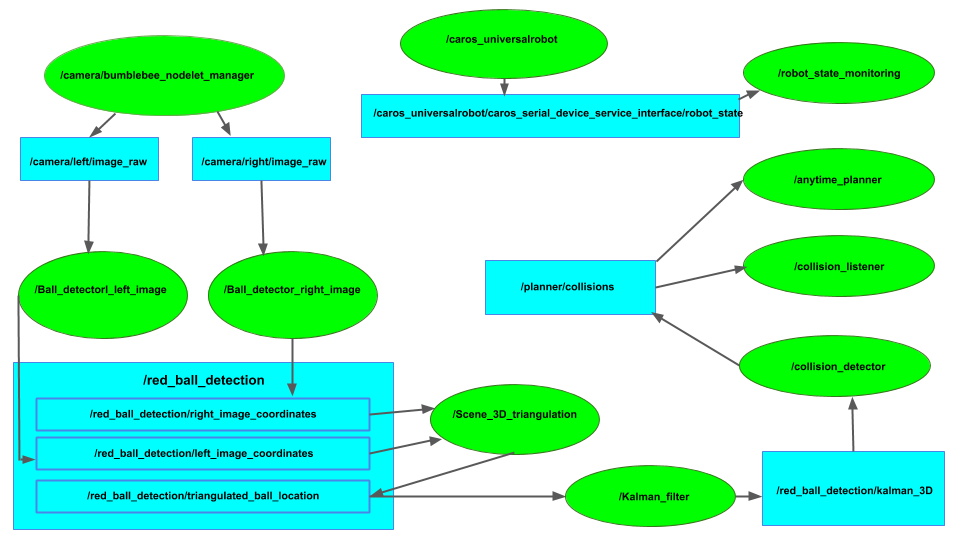
\includegraphics[width=1.1\textwidth]{Images/nodes.png}
    \caption{ROS network. Green ellipses represent nodes whereas blue rectangles represent topics.}
    \label{fig:nodes}
\end{figure}

On the planner side, the first input to the network is the 3D location of the ball tracked in the Kalman node. Until now, all the communications are done using the message type \textit{geometry\_msgs::PointStamped}, which belongs to ROS' API. The collision detector subscribes to the kalman node and uses these three coordinates to update the position of the obstacle and search for potential collisions inside the path calculated and posted by the robot. The collision detector produces boolean messages of the type \textit{std\_msgs::Bool} (also in ROS' API) read by the path planner. While there are no collisions in the path, the robot sticks to the initial plan that was calculated. However, when collisions are detected, the robot stops and replans a new alternative path to reach the goal.

\begin{figure}[ht!]
    \centering
    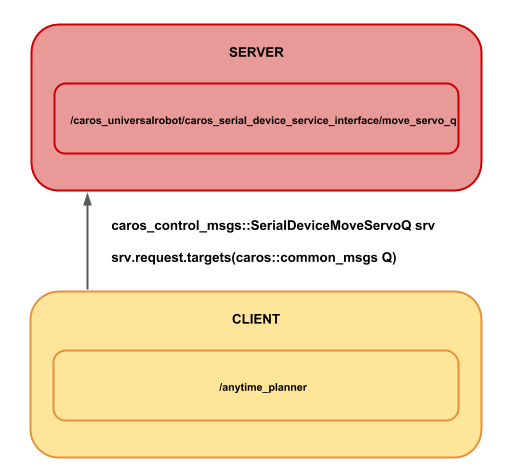
\includegraphics[width=0.6\textwidth]{Images/services.png}
    \caption{CAROS service interface to move the robot by sending Q configuration vectors.}
    \label{fig:services}
\end{figure}

Figure \ref{fig:services} represents the client-server structure of the CAROS serial interface. The planner acts as a client of the \textit{'/move\_servo\_q'} service. When it wants to execute a motion, sends a request with the Q configuration vector that the robot has to reach to the server, which interfaces with the UR controller. 

Now that the flow diagram has been explained, in the next subsections we will explain more in deep how the different nodes were implemented, starting by the vision side.

\subsection{Implementation of the Vision block}

The input to this block are the images that the camera is sending in the ROS network over the topics \textit{'/camera/right/image\_raw'} and \textit{'/camera/left/image\_raw'}. This images correspond to the direct input to the stereo camera, without any type of pre-processing or modification. To be able to use the images, we implemented a bridge between ROS image message type and OpenCV \textit{cv::Mat} image data structure. This operation is done using a function in the ROS API called \textit{cv\_bridge} that easily performs this conversion. With the image converted to \textit{cv::Mat} data type, we applied all the detection techniques to recognize the red ball in the images. Finally, the desired outputs are converted in the last step to the required ROS message types to be exported to other nodes in publishing-subscribing fashion.\\

The code for the vision block was structured in shared libraries in which classes for each separated problem were created: The \textit{'ObstacleDetection'} class to detect the red ball, the \textit{'Stereopsis'} class to perform 3D triangulation and the \textit{'Kalman'} class to track the obstacle in 3D space.

\subsubsection{Ball detection by color segmentation}

The detection function, as well as the subroutine that calls the \textit{cv\_bridge}, is implemented in the \textit{ObstacleDetction.cpp} shared library. Detection is performed individually on the two stereo images, so there are two nodes running the algorithm. These nodes start by calling ROS' \textit{image\_transport} to create subscribers to the \textit{'/image\_raw'} topics. When these images are received, they are converted to \textit{cv::Mat} type and processed. \\

The initial processing steps are Gaussian blurred with a kernel of size 3x3 and converted from BGR to HSV color space. This HSV image is thresholded two times to isolate red colors. The typical range of Hue values for the red is between 160 and 179. Additionally, another threshold is set between 0-10 Hue values to prevent from dark red colors (like maroon or garnet), that could be caused by shadows influencing in the red ball. The two thresholded matrices are combined into one to produce a final binary image.\\ 

The next step is removing noise, in the form of white small dots or shapes apart from the ball, in the binary. To do that, a morphology opening function, with elliptic kernel of size 5, is passed on the image. \\

Finally, to get the center point of the ball, the detector calls the OpenCV function \textit{findContours()}, to get the contour of the ball, and \textit{minEnclosingCircle()} to approximate the minimum circle that covers all the ball area. This last function returns both the center point and the radius of that circle. The last step is to convert the center's pixel coordinates from OpenCV type \textit{$vector<Point2f>$} into \textit{geometry\_msgs::PointStamped}  ROS'  message format to publish them into the topics \textit{'/red\_ball\_detection/right\_image\_coordinates'} and \textit{'/red\_ball\_detection/left\_image\_coordinates'}. \\

\subsubsection{Stereo triangulation}

Stereo triangulation functions are implemented in \textit{Stereopsis.cpp} shared library. The camera intrinsic and extrinsic parameters were estimated during the system's calibration and stored into a \textit{.txt} file that is used by the triangulation node. The first step is to create the projection matrix. Since neither the camera nor the robot base will move from their positions, this matrix is constant all the time. Therefore it is calculated right when the node is run, before it connects to the ROS network of messages. \\

To calculate this projection matrix, as we did in the lectures, two structures were created to store the calibration parameters. The \textit{camera} structure, which stores all the parameters from the calibration \textit{.txt} file, and the \textit{stereoPair} structure, which stores two cameras. This construction is done by the functions \textit{loadCamFromStream()} and \textit{readStereoCameraFile()}. We used the solution provided for the exercise of the second vision lecture of the RoVi2 course \cite{stereopsisExerciseSolution}. \\

With the parameters, function \textit{constructProjectionMat()} constructs a projection matrix as explained in section \ref{sec:tri}, both stored in the \textit{camera} structure.\\

With this matrix already built, the triangulation node subscribes to the detection topics. It is required to have this communication synchronized, to receive coordinates that were detected in both images at the same time. Therefore, the subscribers are not created with the normal procedure, but with the \textit{message\_filters::Subscriber} class. The \textit{Message Filters} library (ROS API) allows managing many messages at once, filtering them by some property. For time synchronization, we use the \textit{timeStamp}. In that way, the triangulation node, when it calls the callback function to process the information coming from the detectors, only uses those messages that come with the same \textit{timeStamp.} As we mentioned above, this synchronization is done using another \textit{message\_filters} function: \textit{message\_filters::TimeSynchronizer}. \\

When the node has already the coordinates of the ball in both images, it performs triangulation using the OpenCV function \textit{triangulatePoints()}, called inside \textit{Stereopsis::calculate\_3D\_location()}, which uses both left and right camera projection matrices and detected points as inputs. It produces a vector that contains the XYZ coordinates of the ball in the real world, with respect to the robot base and in mm. \\

This vector is, finally, transformed again into \textit{geometry\_msgs::PointStamped} message format and published into the topic \textit{'/red\_ball\_detection/kalman\_3D'}. It is important to also synchronize the output message with the inputs. This is done just by coping the \textit{timeStamp} header of the input messages into the output one.

\subsubsection{Kalman filter}

There are three files related to the implementation of the filter:\textit{kalman\_3d.h}, \textit{kalman\_3d.cpp} and \textit{kalman\_ros.cpp}. The firsts files is to create a Kalman Filter class which will contain the methods required to calculate the best estimate point of the ball center. The last one \textit{kalman\_ros.cpp} enables the ROS interface subscriber/publisher to receive and send messages from the \textit{triangulation} to the \textit{collision\_detector} nodes.

In order to implement the algorithm it is used \textit{OpenCV} libraries and \textit(kalman\_template.cpp) provided by the lectures of the course. It is needed to describe the state of the ball that the Kalman Filter will track. In this case is possible to define the state vector as only the position of the ball or adding features such as the velocity and the acceleration of the ball in order to make the estimation more accurate. For this project it is considered the position, velocity and acceleration in the space X,Y and Z as a state vector (see eq. \ref{eq:kf_state} in section \ref{sec:kal}). Furthermore, is needed to describe how many measurements have as input the filter which is the position of the ball's center in the space. Once this is described the Kalman filter is created by \textit{OpenCV} function. However, it is needed to describe a few matrices such as, the transition matrix, which is the relation between the measurements and the state vector. This matrix determines the kinetic equations  by calculating the first and second order derivatives respect to the position of the ball. Additionally, it is required to initialize the covariances matrices of the measurement and process. Which determines the noise level in the process and in the sensors for calculating the best estimate.

Once the initialization is done, the two functions \textit{KALMAN::predict} and
\textit{KALMAN::correct} describes the two-step process mentioned on section \ref{sec:kal}. These functions are called continously in order to predict the position of the ball and correct it based on the measurement received. These two functions are called in another method (\textit{KALMAN::Kalman\_filter\_3D}) which will contain the two-step process along as a \textit{SkipcCorrection} in the case that the ball is missing and the Kalman Filter only needs to predict the state of the object.

Finally, the function \textit{KALMAN::ball\_location\_kf\_callback} which is subscribed to the triangulation node and calls the Kalman function and finally publish te position of the ball in the space.

%explain callback function for the process of receiveing and sending msgs through ros nodes


\subsection{Implementation of the Planner block}
% Talk the WorkCell approach, move the ball, the collision detector... leave the planning function for the end.
In the robotics part there are two main important nodes: the \textit{anytime\_planner} and the \textit{collision\_detector}. This nodes depend not only in the network but also in the RobWorkStudio simulated WorkCell, which contains all the geometries present in the scene (table, computer, ball, robot...). The idea is that to check for collisions, the scene in the WorkCell is updated with the 3D ball coordinates and the robot is moved to see if states in the path collide at some point with the ball or not. Therefore, the simulated scene is updated with the real world information coming from the sensors all the time as well. This bridge between the WorkCell and the robot's actual space is extremely important for the system. \\

To add the geometry of the red ball into it, we created a CAD model of it into the \textit{.xml}, setting the radius and creating it as a movable frame. Then, in the code function that opens and loads the WorkCell into the program, the ball is cast into a movable frame as well, that is able to move it around to with the input coordinates coming from the communication with the Kalman node. The setup of the WorkCell is shown in figures \ref{fig:wc1} and \ref{fig:wc2}. It is worth mentioning that the ball's CAD model is actually bigger than the real ball, considering some clearance for the system to avoid collisions securely. \\

\begin{figure}[ht!]
\centering
\begin{minipage}{.5\textwidth}
  \centering
  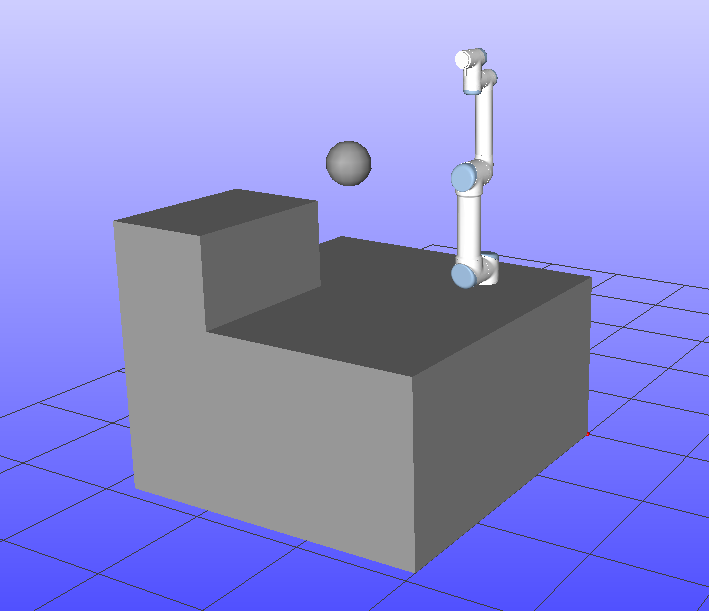
\includegraphics[width=.8\linewidth]{Images/wc1.png}
  \captionof{figure}{Capture from RobWorStudio of the WorkCell setup.}
  \label{fig:wc1}
\end{minipage}%
\begin{minipage}{.5\textwidth}
  \centering
  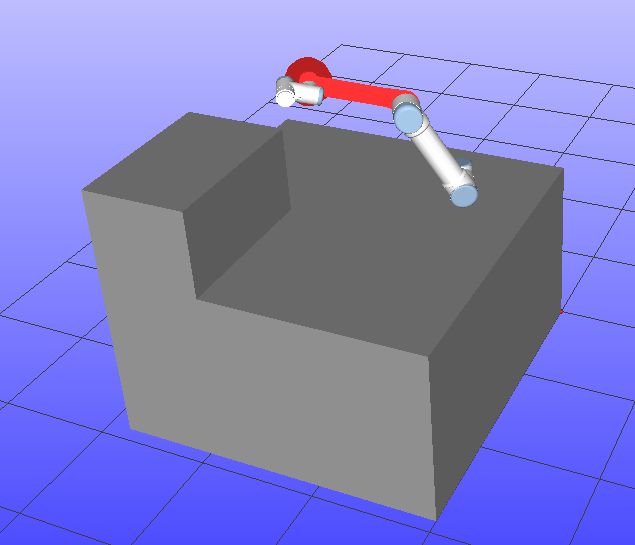
\includegraphics[width=.8\linewidth]{Images/wc2.png}
  \captionof{figure}{Capture of the robot and the ball colliding.}
  \label{fig:wc2}
\end{minipage}
\end{figure}

The subroutine that elaborates search for collisions in the path is not implemented in the planner, but in a separate node. To share the paths that the planner calculates, each time it saves the plan data into a text file that is opened and read cyclically by the collision detection node.\\

The implementation of this part followed the same methodology as in the vision part, creating shared libraries with classes for different scopes. 

\subsubsection{Collision Detector}
% Talk about why we use the plan.txt instead of trajectory.txt to detect collisions
The collision detector is mainly implemented in the class \textit{AnytimePlanning}. This node is subscribed to the topic in which the Kalman node broadcasts the location of the ball. It also reads constantly the paths that the planner calculates from the file were they are being saved and updated.\\

It uses the coordinates of the ball to move the red ball around the scene inside the WorkCell. This is done in using several functions. The first one, \textit{move\_red\_bal()} transforms the coordinates given in \textit{geometry\_msgs::PointStamped} into meters (RobWork's default unit). Then, it moves the ball by using those coordinates to set a new transform matrix for the red ball's movable frame. After moving it, the function \textit{sphere\_strategy()} creates a new collision strategy based on the WorkCell and the ball's location. The last step is to use this strategy to run a \textit{checkCollisions()} functions over the path. We implemented the collision checker to check the path with a reasonably high resolution, not only in the nodes but between them as well. The result of this \textit{checkCollisions()} function is a boolean variable, which is published in the topic \textit{'/planne/collisions'} using the message format \textit{std\_msgs::Bool}. \\

One thing to remark is that, the collision detector can both examine the raw plan calculated by the path planning algorithm, or it can evaluate the trajectory that is later interpolated around this path. This trajectories are generated with time-spaces of 0.05 seconds between consecutive Q vectors. Since the tolerances in the simulated WorkCell are big, and the robot's diameter of its several parts is bigger than in reality, sometimes evaluating the trajectory reports errors. This mistakes are caused by the tolerance issue, which reports that in the simulated WorkCell, self-collisions are detect between robot parts are detected due to the small displacement (0.05 seconds) carried from one node to the next. \\

To overcome this problem, the \textit{plan.txt} file, which contains the raw path prior to be interpolated, is used. This provides enough distance between two consecutive Q vectors to avoid erroneous self-collisions. At the same time, it does not compromise the task by missing collisions, because the nodes in the path are not far enough from each other for that (this last issue, clearly depends on the epsilon parameter of the RRT algorithm). 

\subsubsection{Online planner}
The online path planner node subscribes to the topic published by the collision checker, calculates collision-free paths and works as a client of Caros in order to move the robot. The main idea is to feed the starting and goal configurations to the planner, which calculates a collision-free path and writes it to a file which is read by the collision checker. Whenever the ball is moved in the workcell and a collision appears in the already calculated path, the collision checker publishes the collision status variable accordingly. The path planner node, while iterating from node to node of the path and sending them to the robot, is always listening to the collision status and replans if necessary. After every replanning, a trajectory is interpolated. To send the trajectory to the robot, the state of the robot is constantly monitored. If the state is close enough to the actual node the reach, only then we send the new node of the path. For this purpose, an Euclidian-distance function was implemented.